
  \section{Zielsetzung}
  Dieser Versuch dient der Untersuchung des Relaxionsverhalten
  eines RC-Kreises.
  Hierfür wird die Entladung eines Kondensators betrachtet.
  Zusätzlich wird eine Kondensatorspannung in Hinblick auf die Amplitude
  in Abhängigkeit der Frequenz
  genauer betrachtet.
  Außerdem wird die Phasenverschiebung zwischen Generator-
  und Kondensatorspannung,
  sowie die Funktion als Integrator untersucht.

  \section{Theorie}
  Der Vorgang der Relaxation in einem System tritt auf,
  wenn dieses System aus seinem Ausgangszustand entfernt
  und wieder nicht-oszillatorisch in den selben zurückkehrt.\newline
Für die Betrachtung der Relaxion wird in diesem Versuch
der End- und Aufladevorgang eines Kondensators in einem RC-Glied betrachtet.
Der Aufbau ist in Abbildung \ref{fig:bild1} zu sehen.
\begin{figure}[H]
  \centering
  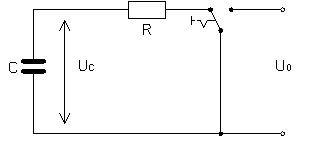
\includegraphics[scale=1.0]{bilder/bild11.png}
  \caption{Schaltung eines RC-Glieds.}
  \label{fig:bild1}
\end{figure}
Für den Endladevorgang folgt aus den Kirchhoffschen Gesetzen,
dass zum Zeitpunkt $ t=0$
\begin{align*}
Q(0)&=CU_0,
\label{eq:RB}
\end{align*}
gilt und nach längerer Zeit
\begin{equation*}
  Q(\infty)=0
\end{equation*}
gilt.
Durch diese Randbedingungen ergibt sich nun die Formel:
\begin{equation*}
  Q(t)= C \cdot U_0\cdot (1-e^{\frac{-t}{RC}})
\end{equation*}
 C ist die Kapazität des Kondensators, R der Widerstand und Q(t) die Ladung zum Zeitpunkt t.\newline
Die Zeitkonstante RC gibt hierbei an wie schnell das System den Endzustand Q(\infty) anstrebt.\newline

Infolgedessen lassen sich Ähnlichkeiten zu mechanischen Systemen finden.\newline
Wird so ein System mit einer Kraft seiner Frequenz angeregt,
steht es in direktem Bezug zu einem angeregten RC-Kreis.\newline
Wird ein RC-Kreises mit einer Wechselspannung
\begin{equation*}
  U(t)=U_0\cos(\omega t)
\label{eq:angeregt}
\end{equation*}
angeregt , kann beobachtet werden, dass eine Phasenverschiebung \phi zwischen der Generator-
und der Kondensatorspannung bei zunehmender Frequenz $\Omega$ auftritt.\newline
Ist die Frequenz $\omega$ viel kleiner als  $\frac{1}{RC}$
 wird die Kondensatorspannung $U_C(t)$ ungefähr gleich der Generatorspannung $U(t)$.\newline
Wird die Freqenz erhöht, entsteht eine Phasenverschiebung zwischen den beiden Spannungen.\newline
Als Formel für die Phasenverschiebung \varphi in Abhängigkeit der Frequenz $\omega$ ergibt sich:
\begin{equation}
  \varphi (\omega) = \arctan(-\omega RC)
\label{eq:phase}
\end{equation}
Für niedrigere Frequenzen geht die Phasenverschiebung gegen dem Wert 0.\newline
Geht die Frequenz gegen unendlich, nährt sich die Phasenverschiebung dem Wert $\frac{\pi}{2}$ an.

Die Beziehung zwischen der Amplitude, der Kondensatorspannung
und der Kreisfrequenz der erregendem Spannung kann durch die Formel
\begin{equation}
A(\omega) = \frac{U_0}{\sqrt{1+\omega^2R^2C^2}}
\label{eq:tiefpass}
\end{equation}
hergestellt werden. Die Amplitude nimmt bei hohen Frequenzen ab.
Aus $\omega \to 0$  folgt, dass $A(\omega)$ gegen $U_0$ geht
und umgekehrt für $\omega \to \infty$ die Amplitude gegen 0 geht.\newline
Dieses Verhalten solcher Tiefpässe ist eben dadurch charakterisiert, dass
Frequenzen mit $\omega \gg \frac{1}{RC}$ immer weiter gesperrt und
$\omega \ll \frac{1}{RC}$ durchgelassen werden.\newline
Es lässt sich außerdem zeigen, dass ein solcher RC-Tiefpass unter der Voraussetzung dass $\omega \gg \frac{1}{RC}$,
also die Frequenz sehr groß ist, die zeitlich veränderliche Spannung $U(t)$ integriert.\newline
Es gilt:
\begin{equation}
  U_C(t) = \frac{1}{RC}\int_0^t U(t')\symup{d}t' \, .
  \label{eq:integrator}
\end{equation}
